\documentclass[12pt,a4paper]{article}
\title{%
  Øving 4 \\
  \large IFYKJT1001 - Fysikk/Kjemi \\
  }
\author{Gunnar Myhre, BIELEKTRO}

\usepackage[utf8]{inputenc}
\usepackage[norsk]{babel}
\usepackage{amsmath}
\usepackage{siunitx}

\usepackage{graphicx}
\graphicspath{ {./images} }

\setlength\parindent{0pt}

\begin{document}
  \maketitle

  \section*{Oppgåve 1}
    \subsection*{a)}
    Den kinetiske energien i ballen er gitt som
    \begin{equation}
      K_{før} = \frac{mv_{før}^2}{2} = \frac{0,226\cdot 22,3^2}{2} = 56,2 J
    \end{equation}
    før kollisjonen, og
    \begin{equation}
      K_{etter} = \frac{mv_{etter}^2}{2} = \frac{0,226\cdot -12,9^2}{2} = 18,8J
    \end{equation}
    etter kollisjonen. Her mangler det
    \begin{equation}
      J = K_{før} - K_{etter} = 37,4[\si{\joule}]
    \end{equation}
    Dette viser også at det er snakk om eit uelastisk støt, sidan $K$ ikkje er bevart.

    \subsection*{b)}
    \begin{equation}
      F=ma \rightarrow F = 0,226\cdot \frac{22,3+12,9}{69,6\cdot 10^{-3}} = 114,2N
    \end{equation}

  \newpage

  \section*{Oppgåve 2}
    \subsection*{a)}
    Sidan krafta frå person A på B er lik krafta frå person B på A kan vi skrive
    \begin{equation}
      F_{A \rightarrow B} = - F_{B \rightarrow A} \rightarrow
      m_1v_1 = - m_2v_2 
    \end{equation}
    denne likninga kjenner vi nå også til mhp. bevaring av bevegelsesmengde. Vi kjenner
    alle dei resterande mengdene og kan finne $v_2$
    \begin{equation}
      v_2 = \frac{m_1v_1}{m_2} = 0,296m/s
    \end{equation}

    \subsection*{b)}
    Vi kan uttrykke den kinetiske energien etter støtet
    \begin{itemize}
      \item $K_1 = \frac{1}{2}m_1v_1^2 = 3,91J$
      \item $K_2 = \frac{1}{2}m_2v_2^2 = 2,59J$
    \end{itemize}
    Sidan vi ikkje kjenner til nokon kinetisk energi før støtet kan vi ikkje
    avgjere om støtet er elastisk eller ikkje. Men om vi antar at personane sto
    i ro (m.a.o. ikkje hadde nokon kinetisk energi $K_1 = K_2 = 0$) og at
    støtet var øyeblikkelig må vi karakterisere det som eit fullstendig uelastisk støt.

  \section*{Oppgåve 3}
    \subsection*{a)}
    Det er to forhold i systemet som er vesentlige for at vi kan rekne ut massen og farta
    til det ukjente atomet
    \begin{itemize}
      \item Bevegelsesmengden er bevart: $m_pv_{p1} + 0 = m_pv_{p2} + xm_pv_{atom}$
      \item Den kinetiske energien er bevart: $K_{p1} + 0 = K_{p2} + K_{atom}$
    \end{itemize}
    Setter inn for kjente mengder for bevegelsesmengdelikninga
    \begin{equation}
      1,5 = 1,2 + xv_{atom}
    \end{equation}
    Setter inn for kjente mengder for energilikninga
    \begin{equation}
      1,5^2 = 1,2^2 + xv_{atom}^2
    \end{equation}
    løyser likningssettet og finner $x = \frac{1}{9}$. Setter inn og vinner dei ukjente
    mengdene.
    \begin{equation}
      m_{atom} = \frac{m_p}{x} \rightarrow m_{atom} = 9m_p
    \end{equation}
    det mest sannsynlege kandidaten med denne massa er beryllium 9.

    \subsection*{b)}
    Farta til atomkjernene som vert trufne er 
    \begin{equation}
      m_p1,5\cdot10^7 = m_p1,2\cdot 10^7 + 9m_pv \rightarrow 
      v = \frac{(1,5-1,2)\cdot10^7}{9} = 3\cdot 10^6
    \end{equation}


  \section*{Oppgåve 4}
    \begin{center}
      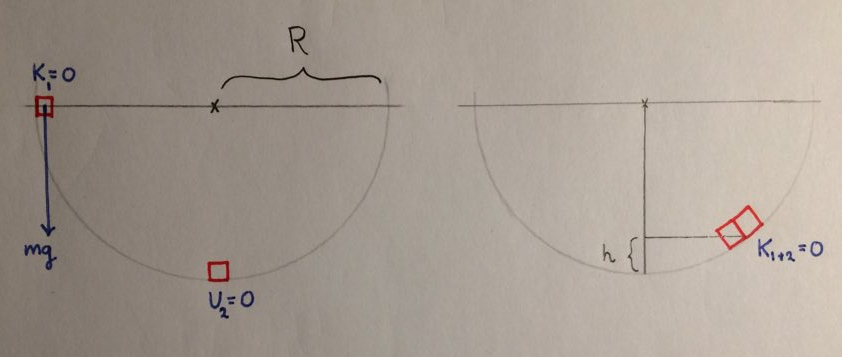
\includegraphics[width=140mm]{04_04}
    \end{center}

    \subsection*{a)}
    På teikninga er all energien i systemet potensiell
    \begin{equation}
      U = m_1gh_1 \rightarrow U = m_1gR
    \end{equation}
    når den øverste boksen når botnen av banen er all energien kinetisk
    \begin{equation}
      U_1 + K_1 = U_2 + K_2 \rightarrow U_1 = K_2 \rightarrow m_1gR = \frac{1}{2}m_1v_1^2
    \end{equation}
    slik får vi eit uttrykk for farten til den øverste boksen i kollisjonsaugeblikket.
    \begin{equation}
      m_1gR = \frac{1}{2}m_1v_1^2 \rightarrow v_1 = \sqrt{2gR}
    \end{equation}
    sidan boksane kolliderer og fortsetter saman som eitt legeme er det snakk om eit
    fullstendig uelastisk støt. Vi kan sette opp bevegelsesbevaringslikning
    \begin{equation}
      m_1v_1 + 0 = (m_1 + m_2)v_2
    \end{equation}
    sidan begge massene er like store
    \begin{equation}
      \frac{mv_1}{2m} = v_2 \rightarrow v_2 = \frac{\sqrt{2gR}}{2}
    \end{equation}
    når dei to boksane når så høgt den kinetiske energien tillater det har dei omgjort all
    sin energi til potensiell energi
    \begin{equation}
      K_{1+2} = U_3 \rightarrow mv_2^2 = 2mgh \rightarrow
      m\frac{2gR}{4} = 2mgh \longrightarrow h = \frac{R}{4}
    \end{equation}

    \subsection*{b)}
    I såfall ville farta $v_2$ vore
    \begin{equation}
      v_2 = \frac{m_1v_1}{m_1+m_2} = \frac{m_1}{m_1+m_2}\sqrt{2gR}
    \end{equation}
    og der kan vi sette $K_{1+2}=U_3$ på denne måten
    \begin{equation}
      \frac{m_1+m_2}{2}v_2^2 = 2(m_1+m_2)gh \rightarrow
      \frac{m_1+m_2}{2} \left( \frac{m_1}{m_1+m_2} \right) ^2 2gR= 2(m_1+m_2)gh
    \end{equation}
    forenkler algebraisk og står igjen med
    \begin{equation}
      h = \left( \frac{m_1}{m_1+m_2} \right) ^2 R
    \end{equation}
    som er alternativ \textbf{D}.

  \section*{Oppgåve 5}
    \subsection*{a)}
    Vinkelhastigheten er den deriverte av $\theta$
    \begin{equation}
      \omega(t) = \theta '(t) = \omega_0 + 2\alpha _0 t, [t \ge 0]
    \end{equation}
    vinkelakselerasjonen er den deriverte av $\omega$
    \begin{equation}
      \alpha(t) = \omega '(t) = 2\alpha _0, [t \ge 0]
    \end{equation}

    \subsection*{b)}
    Med desse startverdiane har vi funksjonen
    \begin{equation}
      \omega(t) = 2,5 + 10,0 t, [t \ge 0]
    \end{equation}
    \begin{itemize}
      \item $\omega(0) = 2,5$
      \item $\omega(5,0) = 52,5$
    \end{itemize}
    gjennomsnittleg vinkelakselerasjon på tidsintervallet $t=[0\rightarrow 5,0]s$ er
    \begin{equation}
      \bar{\alpha} = \frac{\Delta\omega}{\Delta t} = 10,0 [rad/s^2]
    \end{equation}
    gjennomsnittleg vinkelhastighet er
    \begin{equation}
      \bar{\omega} = \frac{\Delta\theta}{\Delta t} = \frac{137,5-0}{5,0} = 27,5[rad/s]
    \end{equation}


  \section*{Oppgåve 6}
    \begin{center}
      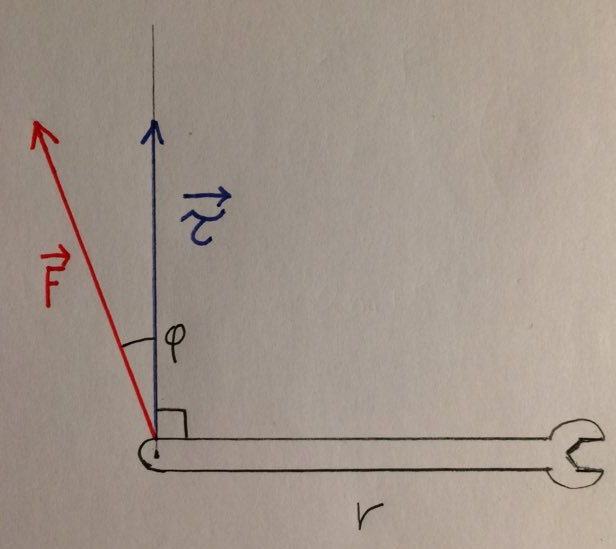
\includegraphics[width=60mm]{04_06}
    \end{center}
    \subsection*{a)}

    Vi kjenner mengdene
    \begin{itemize}
      \item $F = 66,8N$
      \item $\tau = 12,8Nm$
      \item $r = 0,40m$
    \end{itemize}
    Vinkelen finner vi ved å dekomponere vektoren $\vec{F}$
    \begin{equation}
      \tau = rFsin\phi \rightarrow \phi = arcsin \left( \frac{\tau}{rF} \right) = \ang{28,6}
    \end{equation}

  \section*{Oppgåve 7}
    \subsection*{a)}
    Vi må først finne det totale treghetsmomentet til sykkelhjulet. Sidan oppgåveteksten
    behandler systemet som om det ikkje har utstrekning i $z$-retning kan eg bruke
    enklare formlar. Eg beskriver felgen som ein jevn ring, eikene som tri tynne stag
    (parallellforskyve ut til trinsas periferi) og trinsa som ei tynn, solid plate.
    \begin{itemize}
      \item $I_{felg} =\frac{1}{2}m(r_1^2+r_2^2) = 9,62\cdot 10^{-2}[kgm^2]$
      \item $I_{eike} =I_{CM}+md^2 = \frac{1}{3}mL^2 + md^2 = 4,83 \cdot10^{-3}[kgm^2]$
      \item $I_{trinse} =\frac{1}{2}mr^2 = 8,0\cdot10^{-5}[kgm^2]$
    \end{itemize}
    Merker at lengdene må vere i meter. Det totale treghetsmomentet er
    \begin{equation}
      I_{hjul} = I_{felg} + 3I_{eike} + I_{trinse} = 0,11kgm^2
    \end{equation}

    \subsection*{b)}
    Krafta som loddet utfører på hjulet gjev eit dreiemoment som står tangentielt på trinsa
    \begin{equation}
      \tau = rF = 0,04m\cdot0,5kg\cdot9,81m/s^2 = 0,2Nm
    \end{equation}
    vi kan finne vinkelakselerasjonen vha. Newtons andre lov på rotasjonsform
    \begin{equation}
      (\Sigma \tau_z)_{ytre} = I\cdot \alpha_z \longrightarrow \alpha = \frac{\tau}{I}
    \end{equation}
    vi kan omgjere $\alpha = \frac{a}{r}$ og finne akselerasjonen til loddet
    \begin{equation}
      a = \frac{\tau r}{I} \rightarrow a = 0,072m/s^2
    \end{equation}

    \subsection*{c)}
    Bruker den tidlause bevegelseslikninga for konstant akselerasjon.
    Etter å ha falt $1,2m$ har loddet farta.
    \begin{equation}
      v^2 = 2as \rightarrow v^2 = 2\cdot0,072\cdot1,2\rightarrow v = 0,416m/s
    \end{equation}
    gjer om til vinkelhastighet 
    \begin{equation}
      \omega = \frac{v}{r} = \frac{0,416}{0,04} = 10[rad/s]
    \end{equation}
    




\end{document}
